\chapter{PCA on spectral data}
\label{ch:spectral-PCA}



%\begin{marginfigure}
%   \centering
%  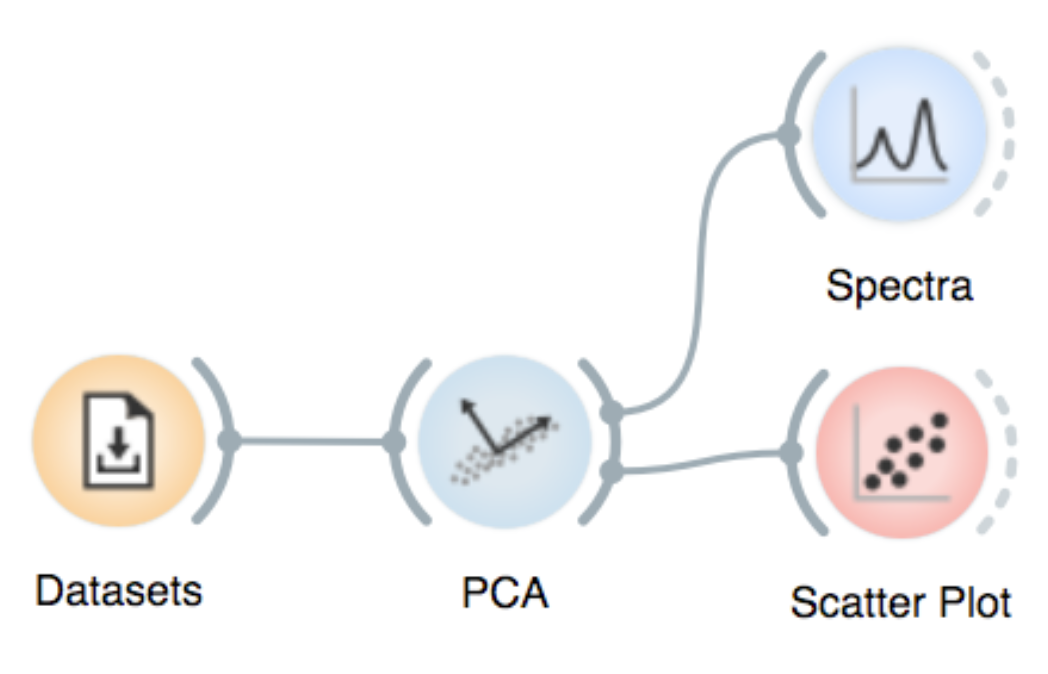
\includegraphics[width=\linewidth]{graphics/ch-spectral_PCA/spectral_PCA-fig1.png}%
%  \caption{Start with this simple workflow.}
%  \label{fig:spectral-PCA-fig1}
%\end{marginfigure}


% MARKO: an alternative side image addition
% I think we should avoid Figures unless we want to add captions; we can add images directly
% We probably need to add figure environments so that they are not counted and do not start with "Figure X" - We only need them for comments.

\begin{wrapfigure}{o}{0.5\textwidth}
    \centering
    \vspace{-2cm}
    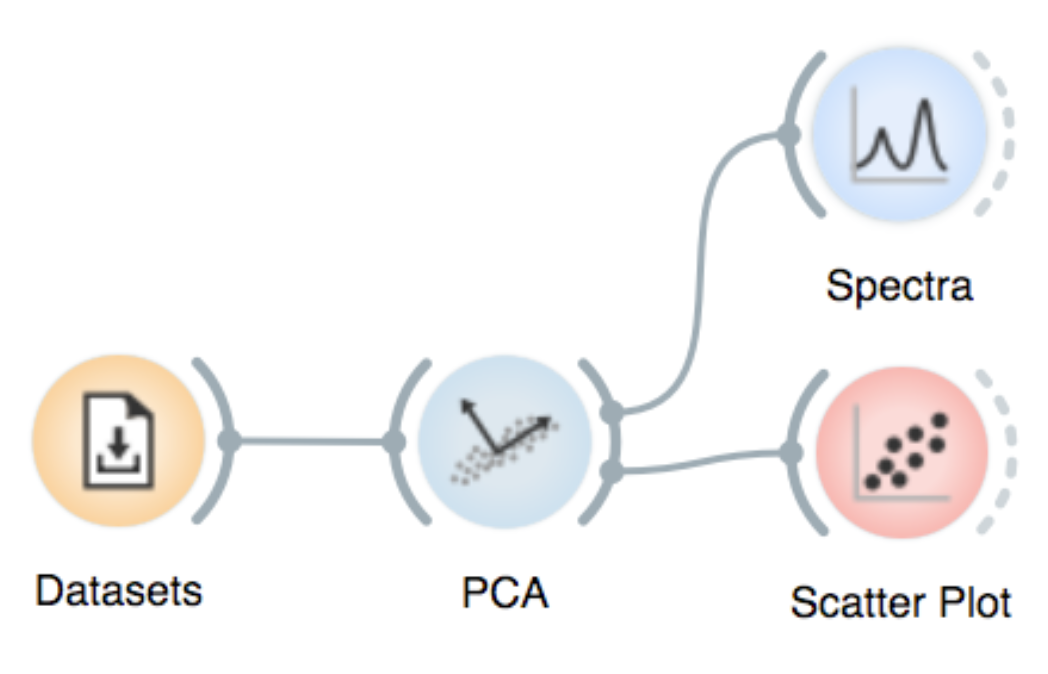
\includegraphics[width=0.55\textwidth]{graphics/ch-spectral_PCA/spectral_PCA-fig1.png}
\end{wrapfigure}

In this lesson we will explore the capabilities of \mutation\ for principal component analysis (PCA) on spectroscopy data. As usual, we will use the Liver Spectroscopy dataset. Connect \textit{Datasets} to the \textit{PCA} widget, choose the first 5 principal components and then connect \textit{PCA’s} default output, "Transformed Data", into the \textit{Scatter Plot}. 

We see that the first two principal components separate majority compounds in that part of the tissue well. 


% MARKO: Here is how I propose how to add images.
% I prefer not making combined screenshots.
% The original images can be copied from the pages file directly, if it is saved as a package: File -> Advanced -> Change file type -> Package.
% Then we can open the package in finder. Images there have funny names, but we can rename one by one. When the names are nice, they can be copied in the correct chapter and added into the document with code like below. 
% This also allows us to take images without any loss of quality and we can also scale them so that combined images always have the same resolution.
% Here I made it just for one example. If you agree, let's do them all.

% FERI: I like this approach a lot. As I said in my email, let's try to combine all these package functionality into our own figure environment if possible, to simplify the figure insertion... For now I will use this
\begin{figure}[h]
\hspace{-1cm}\stackinset{r}{-0.4\linewidth}{t}{+0.1\linewidth}
  {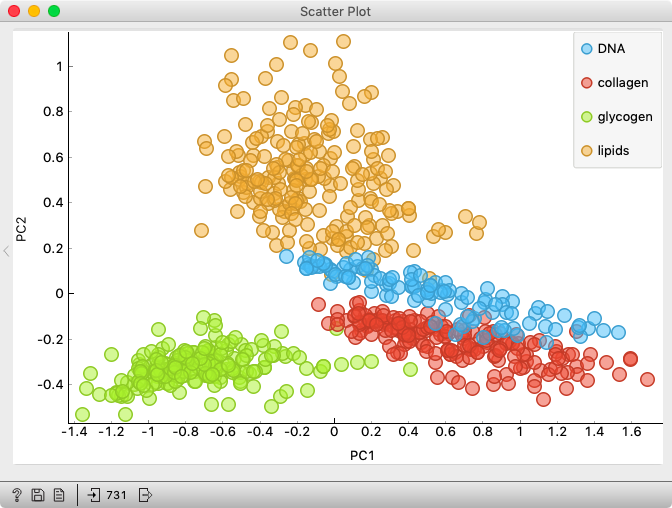
\includegraphics[scale=0.4]{graphics/ch-spectral_PCA/scatterplot.png}}
  {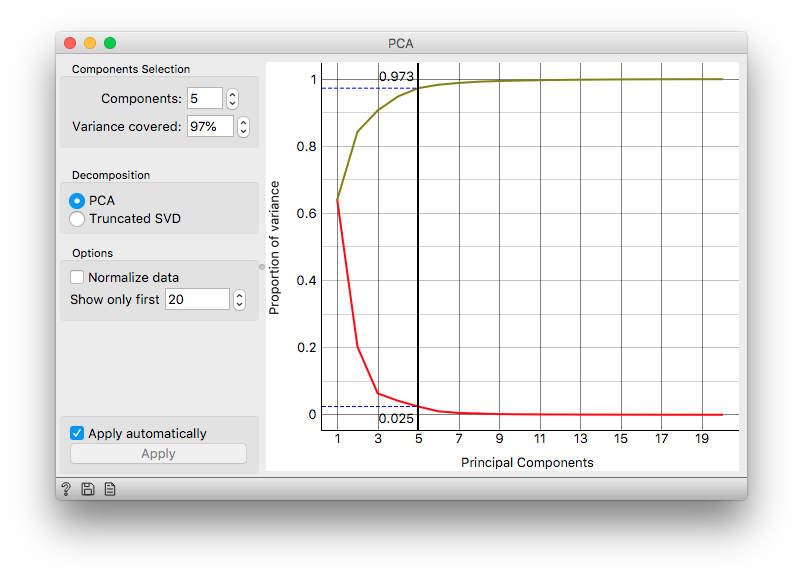
\includegraphics[scale=0.4]{graphics/ch-spectral_PCA/pca.png}}
  \caption{We chose not to normalize variables in \textit{PCA}. Why?}
  \label{fig:spectral-PCA-fig2}
\end{figure}

\begin{wrapfigure}{o}{0.8\textwidth}
  \centering
  \vspace{-0.5cm}
  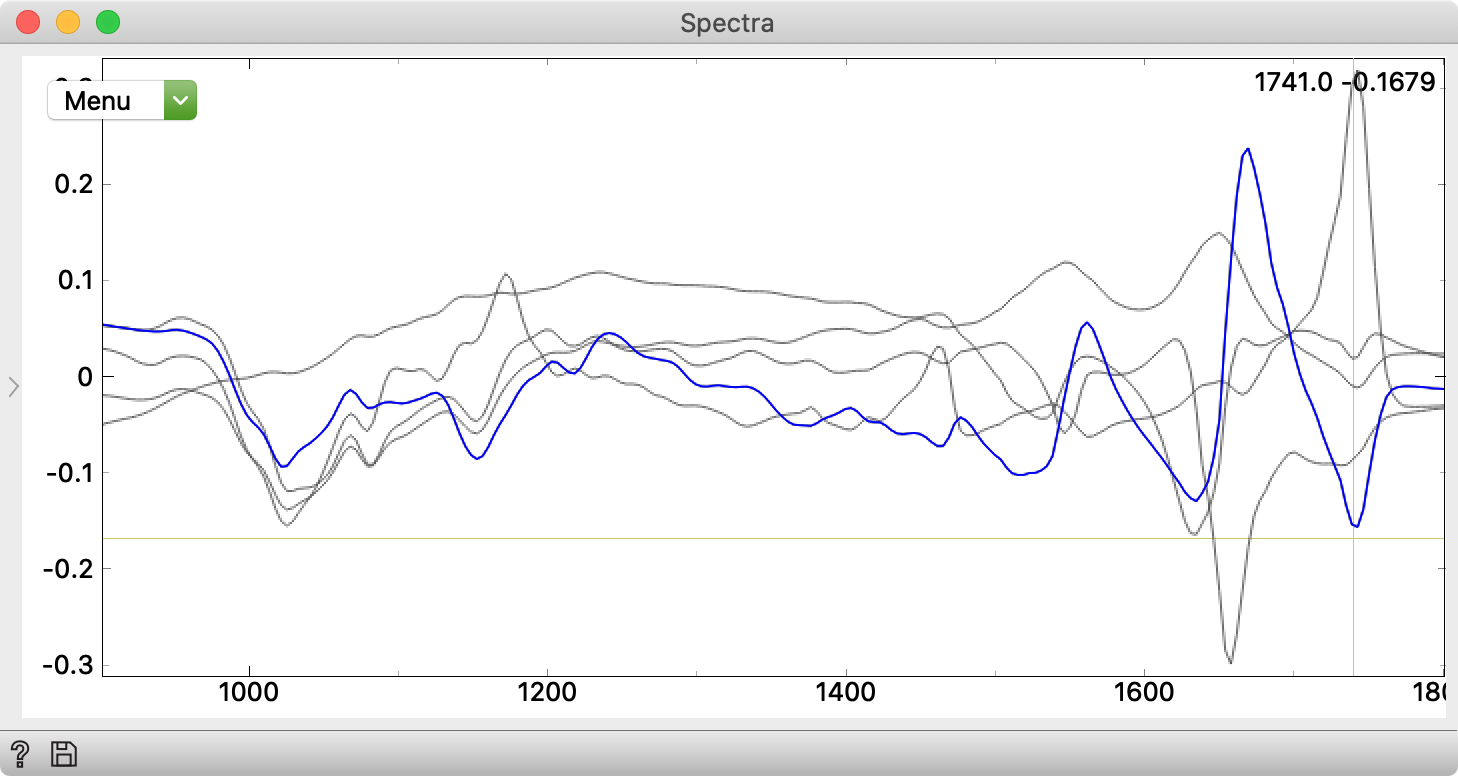
\includegraphics[width=0.8\textwidth]{graphics/ch-spectral_PCA/spectral_PCA-fig3.png}%
  \caption{The curve under the cursor is highlighted. A tooltip will appear after some time. If clicked, the curve will be selected.}
  \label{fig:spectral-PCA-fig3}
\end{wrapfigure}

To see what different principal components represent, connect \textit{PCA’s} "Components" output (be careful, \textit{PCA} has 3 outputs) into \textit{Spectra}. Wondering which principal component is highlighted in the following screenshot? Wait for the tooltip...

Let's extend our workflow. In the next example, we are also using the “Data Subset” input. The \textit{Scatter Plot} and \textit{Spectra (2)} widgets on the right get both the whole data and a subset of it.

\begin{wrapfigure}{o}{0.7\textwidth}
  \centering
%   \vspace{-2cm}
  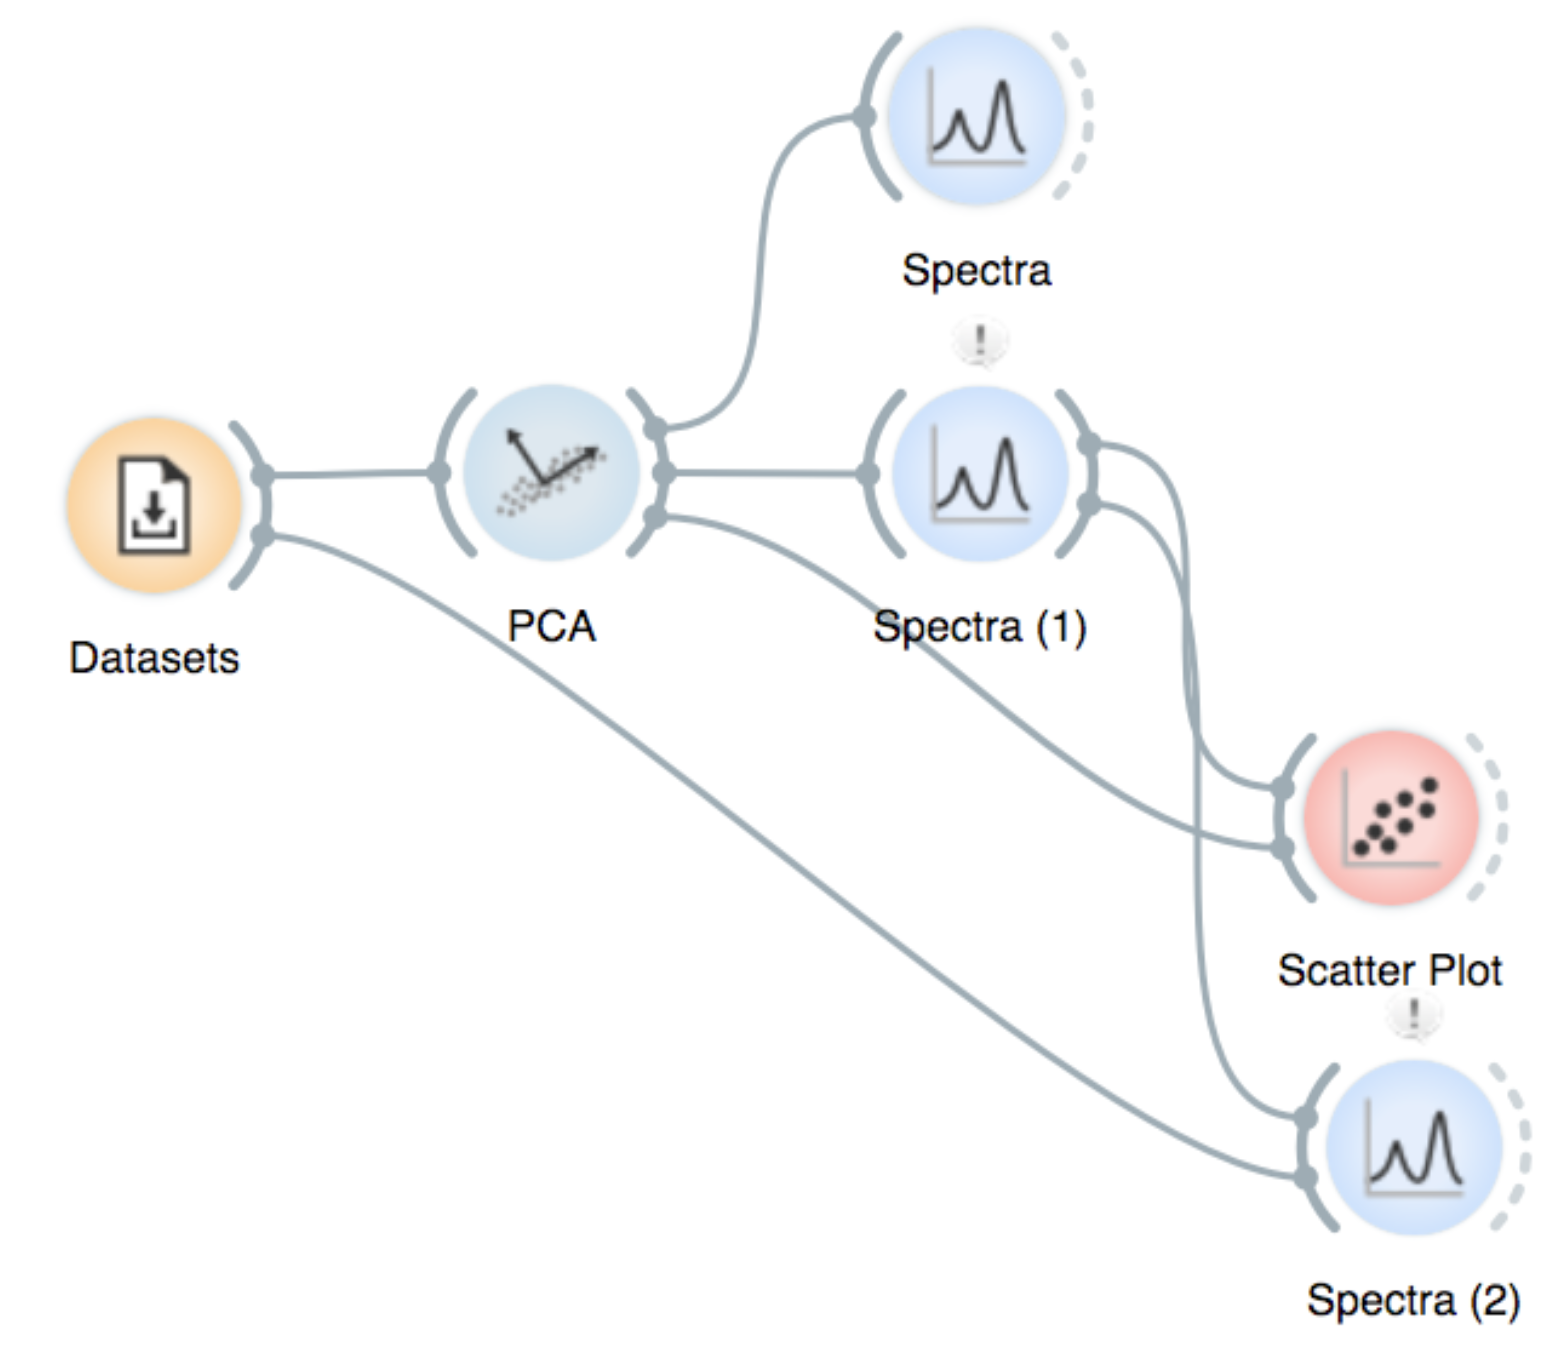
\includegraphics[width=75mm]{graphics/ch-spectral_PCA/spectral_PCA-fig4.png}%
  \label{fig:spectral-PCA-fig4}
\end{wrapfigure}

If we connect the \textit{PCA} (Transformed data output) to \textit{Spectra (1)}, we see each transformed spectrum on a line plot. As we can see, some classes have outliers. 

To find out more, select one of them: move your mouse cursor to a curve -—it will be highlighted—- and click it. The selected curve changes to a dotted line and is sent to the output. Then, connect that output to a \textit{Scatter Plot} and another \textit{Spectra} widget (both to its Data Subset inputs). We can then see the spectrum in the original space (\textit{Spectra (2)} widget) and the space of principal components (\textit{Scatter Plot}).

\begin{figure*}[h]
%   \centering
  \vspace{3cm}\stackinset{r}{0pt}{t}{+0.35\textwidth}
  {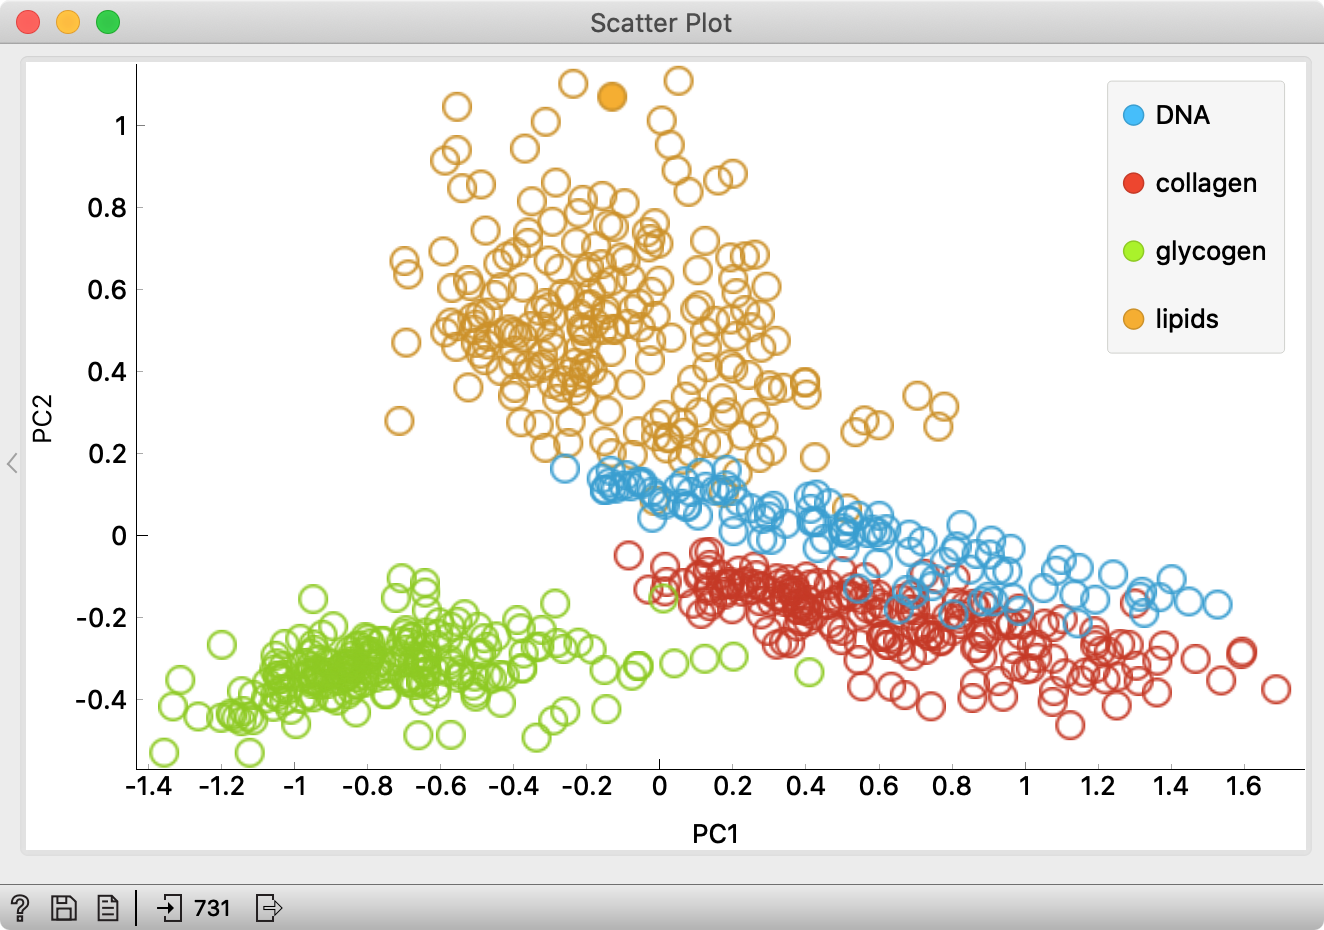
\includegraphics[width=0.48\textwidth]{graphics/ch-spectral_PCA/spectral_PCA-fig6.png}}
  {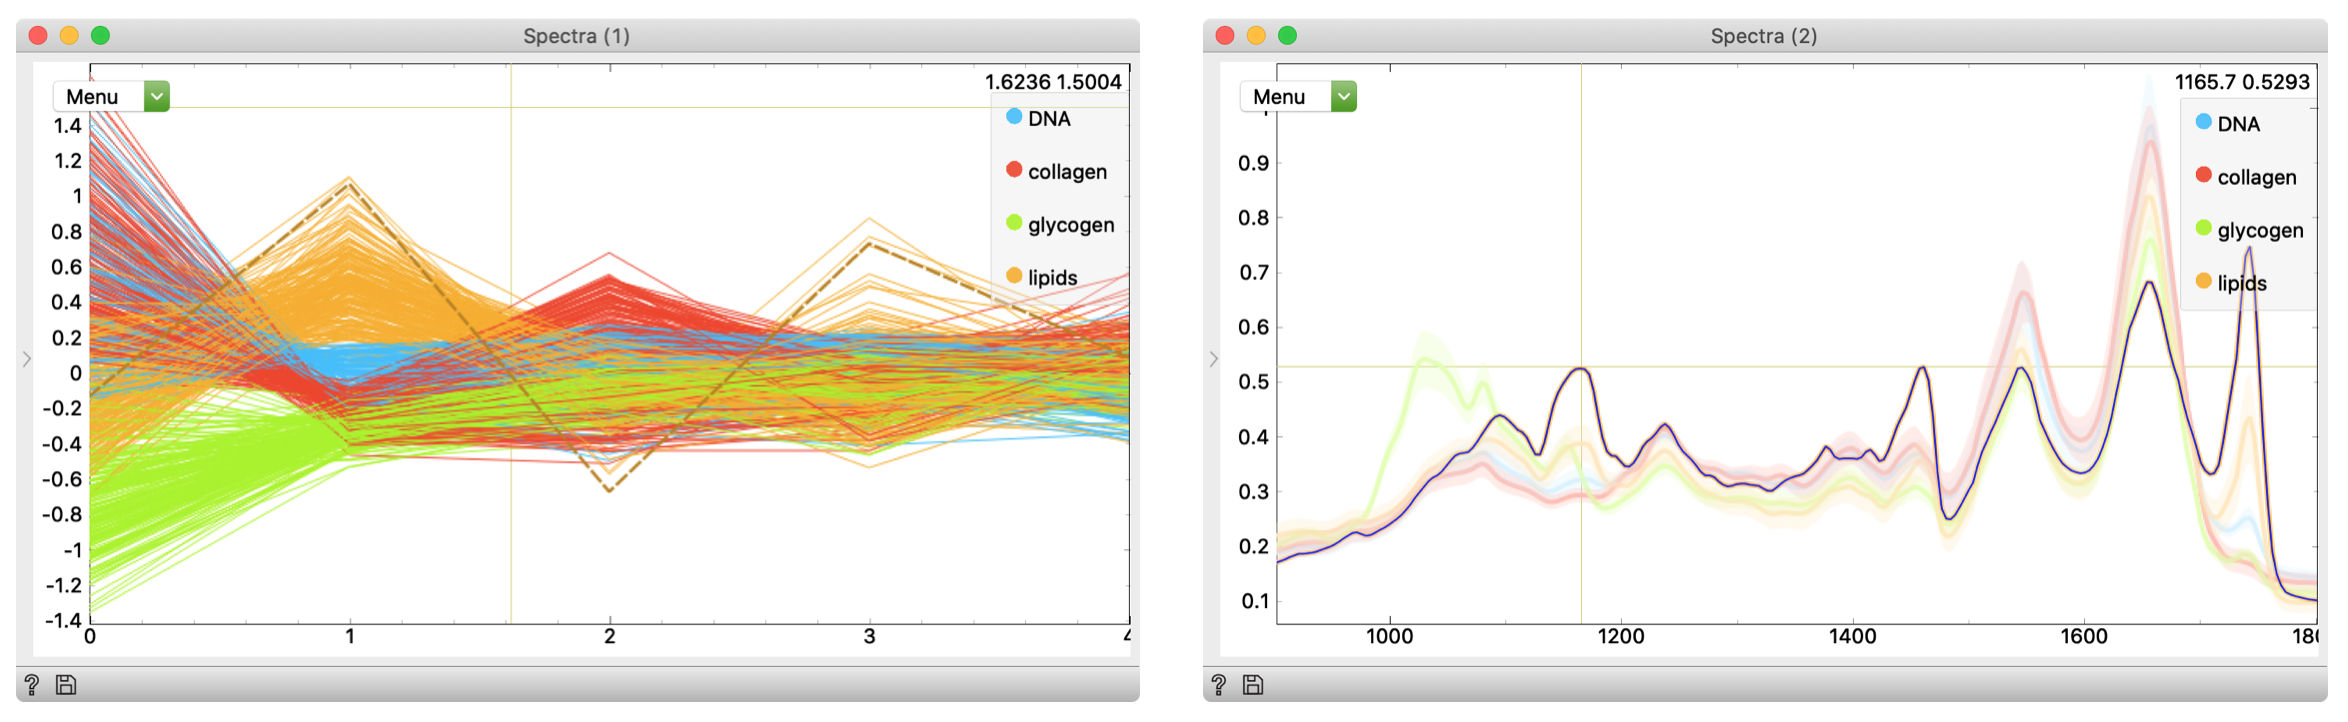
\includegraphics[width=\textwidth]{graphics/ch-spectral_PCA/spectral_PCA-fig5.png}}
  \vspace{-3.5cm}
  \caption{The selected spectrum's curve on the left is drawn with a dashed line and the corresponding original spectrum is highlighted on the right. \textit{Scatter Plot} shows the position of the selected spectrum in the PCA space.}
  \label{fig:spectral-PCA-fig5}
\end{figure*}

%% Text boxes that stretch for the whole width of the page would probably solve this issue. Then we could place the corresponding text with the figure and they wouldn't move relative to each other. Inside the textbox we can still keep the style of the main document.